\chapter{Results}
\label{ch:results}

This chapter presents the experimental evaluation of the fine-tuned SimLingo model on the QLabs roundabout scenario and compares it against a LiDAR-based adaptive cruise control (ACC) baseline. Both controllers are evaluated on the same test matrix using identical metrics (described in \Cref{ch:evaluation}). All SimLingo evaluation runs reported in this chapter use the final checkpoint from the QLabs fine-tuning run (\texttt{epoch\_14.pt}, i.e., epoch~14 of 15, stored under \path{simlingo/outputs/2025_11_26_18_06_21_qlabs_roundabout_finetune/checkpoints/}).

\section{Training convergence}
\label{sec:training-convergence}

\Cref{fig:training-losses} shows the training and validation loss curves over 15~epochs of QLabs fine-tuning. The three loss components---route loss, speed-waypoint loss, and their sum (total loss)---are each Smooth-$\ell_1$ losses on the predicted vs.\ ground-truth waypoints, as defined in \Cref{sec:training-losses}. All three decrease rapidly in the first 3--5~epochs before flattening, indicating that the model learns the QLabs driving distribution relatively quickly. The language loss remains near zero throughout training because no natural-language supervision is provided (see \Cref{sec:final-dataset-scope}). The learning rate follows a one-cycle schedule with 5\% warmup, decaying smoothly after the initial ramp.

\begin{figure}[htbp]
  \centering
  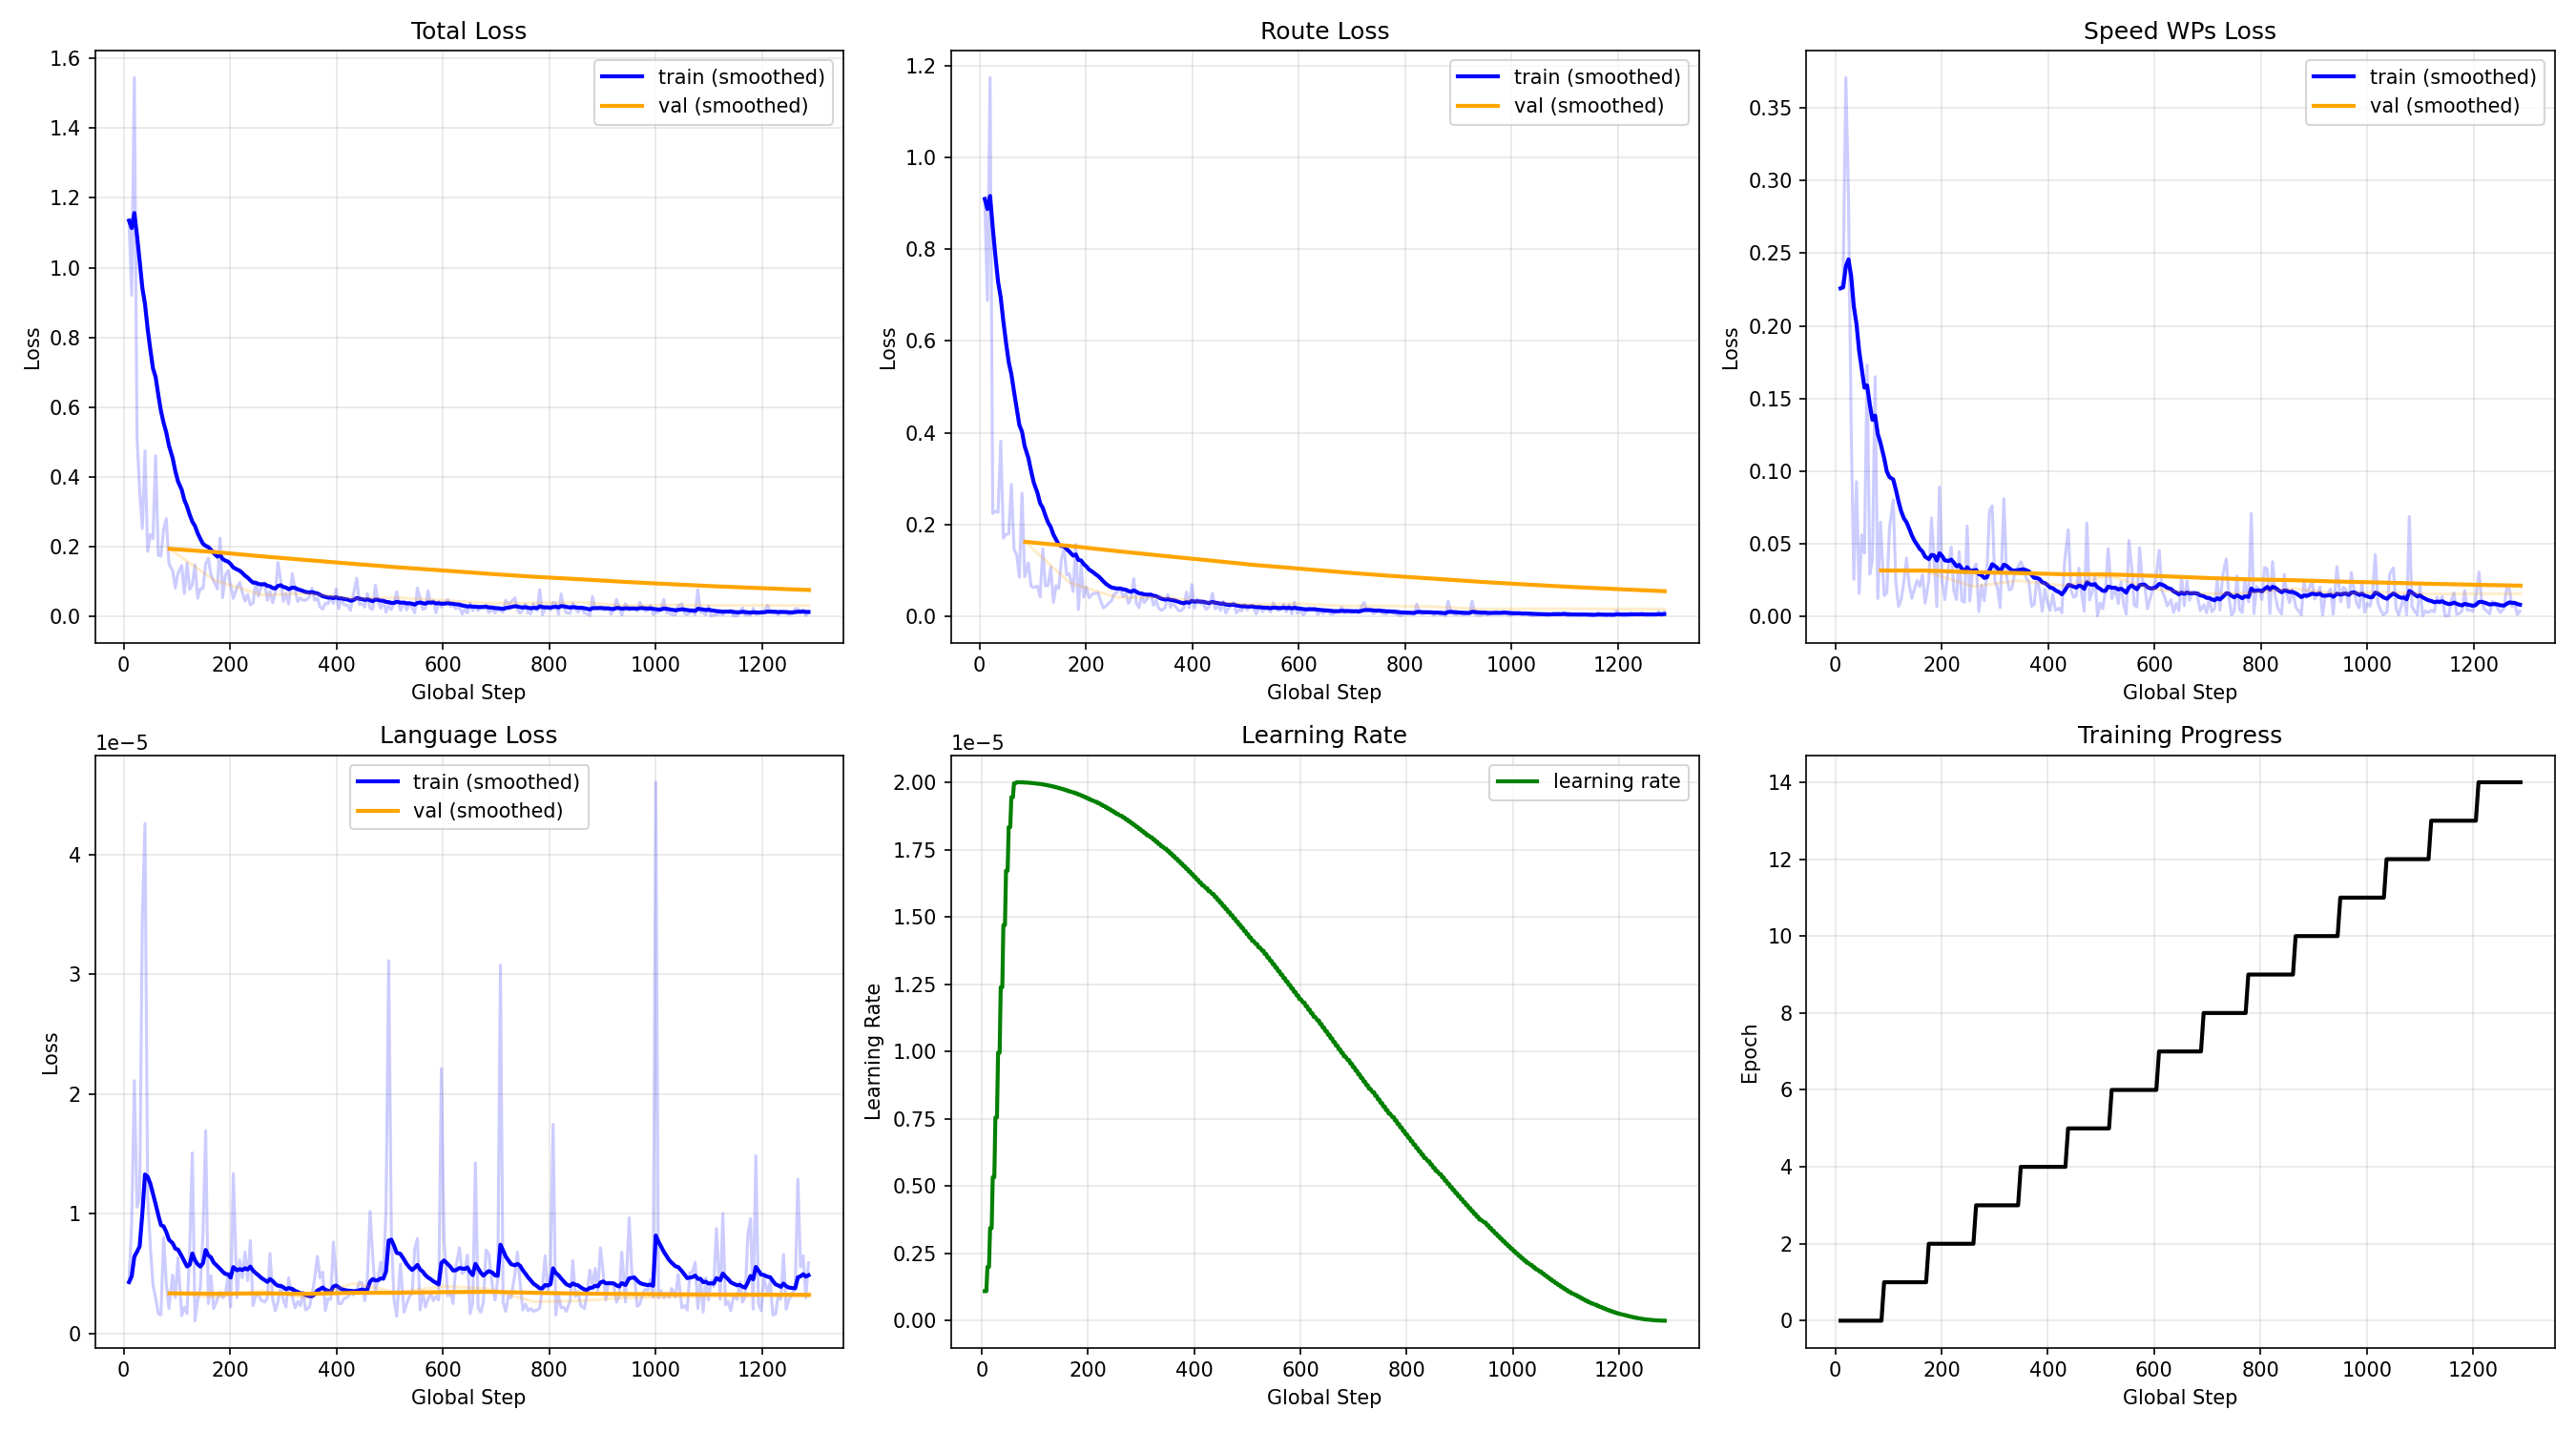
\includegraphics[width=\textwidth]{metrics.png}
  \caption{Training loss curves over 15~epochs. Top row (left to right): total loss, route loss, speed waypoints loss. Bottom row: language loss, learning rate schedule, epoch progress. Blue: training (smoothed); orange: validation (smoothed); faint traces: raw values.}
  \label{fig:training-losses}
\end{figure}

\Cref{fig:ade-curve} shows the Average Displacement Error (ADE) for both the learned policy and the expert demonstrations, evaluated on the validation split across all 15~epoch checkpoints. ADE is computed as the mean point-to-polyline distance: for each predicted trajectory point (10~speed waypoints for the policy, 11~ego-position waypoints for the expert), the perpendicular distance to the nearest segment of the ground-truth route polyline (20~points) is calculated, and the distances are averaged. This metric handles the differing number of trajectory and route points without resampling artifacts by measuring how closely each trajectory follows the planned route regardless of spatial extent.

The expert demonstration ADE is $0.087$~m, representing how closely the human teleoperator followed the planned route. The policy ADE drops from $0.114$ at epoch~0 to approximately $0.085$ by epoch~11---a 25\% reduction---converging toward the expert baseline. After epoch~1 the policy already operates near expert-level performance, with the remaining epochs producing marginal gains. The final ADE of ${\sim}0.085$~m means the model's predicted trajectories deviate less than 9~cm on average from the planned route, comparable to the expert's own deviation and well within the QCar~2's lateral footprint.

\begin{figure}[htbp]
  \centering
  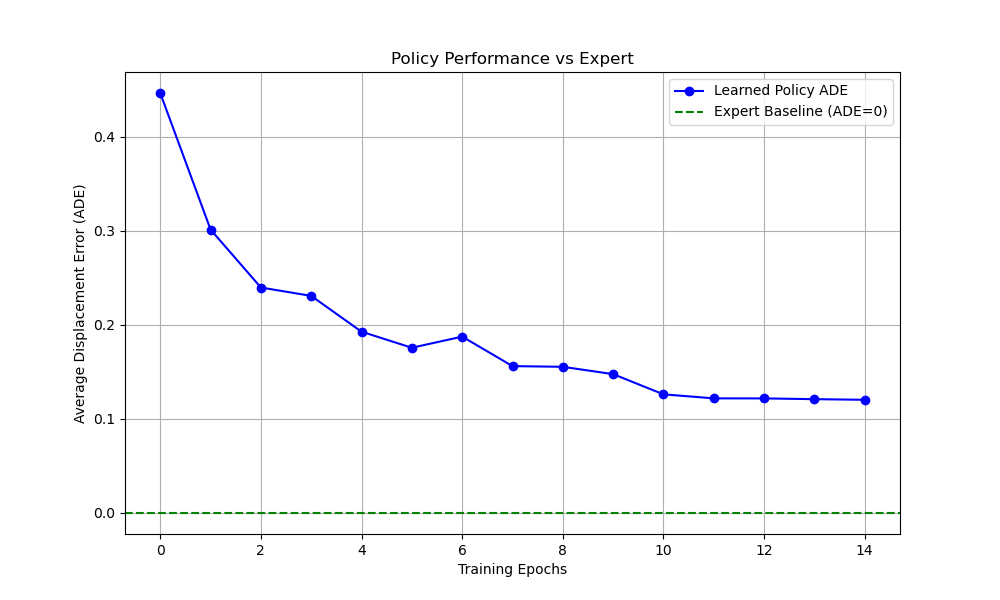
\includegraphics[width=0.75\textwidth]{policy_vs_expert_curve.png}
  \caption{Average Displacement Error (ADE) across training epochs. ADE is measured as the mean point-to-polyline distance from each trajectory point to the nearest segment of the ground-truth route. The learned policy (blue) converges from $0.114$ toward the expert demonstration baseline (red dashed, ADE${=}0.087$). The green dashed line represents the ground-truth route (ADE${=}0$).}
  \label{fig:ade-curve}
\end{figure}

\section{Baseline route following (no obstacles)}
\label{sec:baseline-results}

\Cref{tab:baseline-comparison} summarizes the performance of both controllers on the clean roundabout route (no obstacles), averaged over 5~runs each. Both controllers achieve high route coverage, confirming that each can reliably navigate the full roundabout under nominal conditions. SimLingo achieves lower average lateral deviation (0.056~m) than the ACC baseline (0.261~m), reflecting the fact that the learned policy was trained to replicate expert trajectories recorded along this exact route. The ACC baseline uses a generic pure-pursuit algorithm with a 4.5~m lookahead, which produces smoother but less route-adherent trajectories due to corner-cutting on curved segments. SimLingo takes longer per run (68~s vs 43~s) because it operates at 4~Hz inference with a lower average speed, whereas the ACC baseline cruises at a fixed 2.0~m/s.

\begin{table}[htbp]
\centering
\caption{Baseline route following (no obstacles), 5~runs per controller.}
\label{tab:baseline-comparison}
\begin{tabular}{lcccc}
\toprule
Controller & Coverage (\%) & Avg Lat.\ Dev.\ (m) & Max Lat.\ Dev.\ (m) & Avg Time (s)\\
\midrule
SimLingo & \textbf{\input{figures/val_sim_baseline_coverage}} & \textbf{\input{figures/val_sim_baseline_avgdev}} & \textbf{\input{figures/val_sim_baseline_maxdev}} & \input{figures/val_sim_baseline_time} \\
ACC Baseline & \input{figures/val_acc_baseline_coverage} & \input{figures/val_acc_baseline_avgdev} & \input{figures/val_acc_baseline_maxdev} & \textbf{\input{figures/val_acc_baseline_time}} \\
\bottomrule
\end{tabular}
\end{table}

\section{Obstacle avoidance results}
\label{sec:obstacle-results}

\Cref{tab:obstacle-results} reports the per-scenario and per-controller metrics for the five obstacle placement variants, with 2~runs each. The test matrix evaluates whether each controller can (a)~detect the static obstacle, (b)~stop safely before reaching it, and (c)~avoid collision. Note that the ``Collision'' and ``Stopped'' columns are reported independently: a run may show both collision and stopped, which indicates that the vehicle decelerated to near-zero speed but made low-speed bumper contact with the obstacle before fully stopping. These runs are classified as failures (any obstacle contact constitutes a collision), but the stopping behavior is reported separately to show that the model did attempt to stop.

\begin{table}[htbp]
\centering
\caption{Obstacle scenario results. Each variant is tested with 2~runs per controller.}
\label{tab:obstacle-results}
\resizebox{\textwidth}{!}{%
\begin{tabular}{llccccc}
\toprule
Scenario & Controller & Coverage (\%) & Collision & Stopped & Stop Dist.\ (m) & Avg Lat.\ Dev.\ (m) \\
\midrule
\input{figures/obstacle_results_table_rows}
\end{tabular}%
}
\end{table}

\Cref{fig:pass-fail-summary} provides a visual summary of the pass/fail outcomes across all scenarios and controllers. SimLingo achieves an overall pass rate of 60\% (9/15 runs), which includes 5/5 baseline runs and 4/10 obstacle runs. Note that the overall 60\% pass rate and the 60\% collision rate shown in \Cref{fig:safety-comparison} are computed over different denominators: the pass rate includes all 15~runs (baseline + obstacle), whereas the collision rate is computed over the 10 obstacle runs only (6/10 collisions).

\begin{figure}[htbp]
  \centering
  
\includegraphics[width=0.85\textwidth]{pass_fail_summary.png}
  \caption{Pass/fail summary across all 15~runs (5~baseline + 10~obstacle) for SimLingo and ACC baseline. The total pass rate includes baseline runs; see \Cref{fig:safety-comparison} for obstacle-only safety metrics.}
  \label{fig:pass-fail-summary}
\end{figure}

\section{Comparative analysis}
\label{sec:comparative-analysis}

\Cref{fig:route-coverage} compares route coverage across all scenarios. On the clean baseline, both controllers achieve near-complete coverage. On obstacle scenarios, coverage diverges: the ACC baseline consistently stops 5--8.5~m before the obstacle due to its fixed LiDAR detection cone, whereas SimLingo's stopping distance varies with approach speed and obstacle visibility (see \Cref{sec:results-discussion}). Note that higher coverage in obstacle scenarios does not indicate better performance---it primarily reflects shorter stopping distances and, in the case of Variant~5, a complete failure to stop. Coverage is therefore most informative on the obstacle-free baseline; for obstacle scenarios, the safety metrics in \Cref{fig:safety-comparison} are the appropriate comparison.

\begin{figure}[htbp]
  \centering
  
\includegraphics[width=0.85\textwidth]{route_coverage_comparison.png}
  \caption{Route coverage comparison across scenarios. Error bars show standard deviation across runs.}
  \label{fig:route-coverage}
\end{figure}

\Cref{fig:safety-comparison} compares safety metrics across the 10 obstacle runs only (2~runs $\times$ 5~variants per controller), excluding the baseline. SimLingo shows a 60\% collision rate (6/10 obstacle runs), corresponding to the 40\% obstacle pass rate visible in the per-scenario breakdown of \Cref{fig:pass-fail-summary}. The stop success rate and average stopping distance further characterize how each controller responds to static obstacles.

\begin{figure}[htbp]
  \centering
  
\includegraphics[width=0.85\textwidth]{safety_comparison.png}
  \caption{Safety metrics comparison for the 10 obstacle runs only (excludes baseline): collision rate (lower is better), stop success rate (higher is better), and average stopping distance.}
  \label{fig:safety-comparison}
\end{figure}

\Cref{fig:lateral-deviation} compares average lateral deviation from the route centerline across scenarios. SimLingo achieves lower average deviation (0.03--0.09~m) than the ACC baseline (0.25--0.38~m) on most scenarios. This difference is explained by the trajectory overlays in \Cref{fig:trajectory-overlays}: on the roundabout curve, the ACC baseline (orange dashed) consistently tracks \emph{inside} the route centerline (black dashed) due to pure-pursuit corner-cutting with a 4.5~m lookahead, whereas SimLingo (blue solid) follows the route more closely because it was trained on expert demonstrations recorded along this exact path. On the straight sections of the route, both controllers track the centerline with similar precision (${\sim}0.06$~m). The overall difference in the bar chart is dominated by the curved portion of the route, where the ACC deviates 0.4--0.7~m from the centerline. The exception is Variant~5, where SimLingo's deviation increases to 0.28~m as the vehicle swerves through the obstacle zone.

\begin{figure}[htbp]
  \centering
  
\includegraphics[width=0.85\textwidth]{lateral_deviation_comparison.png}
  \caption{Average lateral deviation from route centerline by scenario. The ACC baseline's higher deviation is primarily caused by pure-pursuit corner-cutting on the roundabout curve, as visible in \Cref{fig:trajectory-overlays}.}
  \label{fig:lateral-deviation}
\end{figure}

\Cref{fig:trajectory-overlays} shows bird's-eye trajectory overlays for each obstacle variant. On the roundabout curve (top-right arc of each subplot), the ACC trajectories (orange dashed) are visibly offset inward from the route centerline (black dashed), confirming the lateral deviation pattern in \Cref{fig:lateral-deviation}. SimLingo trajectories (blue solid) follow the route centerline more closely on curves but exhibit higher-frequency oscillations compared to the smooth ACC paths. The stopping positions relative to the obstacle markers (red squares) are also visible: SimLingo stops cleanly before the obstacle in Variants~1 and~3, decelerates and stops near the obstacle (with low-speed bumper contact) in Variants~2 and~4, while in Variant~5 the blue trajectory extends through the obstacle location.

\begin{figure}[htbp]
  \centering
  
\includegraphics[width=\textwidth]{trajectory_overlays.png}
  \caption{Trajectory overlays for each obstacle variant. Route centerline (black dashed), SimLingo trajectories (blue solid), ACC trajectories (orange dashed), and obstacle positions (red squares).}
  \label{fig:trajectory-overlays}
\end{figure}

\section{Discussion}
\label{sec:results-discussion}

The results demonstrate that the fine-tuned SimLingo model can navigate the roundabout route and respond to static obstacles using only camera input, without access to LiDAR. The model achieves a 40\% obstacle pass rate (4/10 runs), with contact-free stops on Variants~1 and~3, low-speed contact on Variants~2 and~4, and a complete failure on Variant~5. Several factors explain the observed performance.

\paragraph{Low speed at encounter enables clean stops.}
The SimLingo model stops cleanly (no bumper contact) for Variant~1 (early roundabout) and Variant~3 (roundabout exit), where the vehicle has not yet reached high speed at the time of obstacle encounter. In Variant~1, the car is still accelerating through the initial straight segment and traveling below 1.5~m/s when it perceives the obstacle, leaving sufficient distance to decelerate and stop at approximately 6.8~m from the obstacle center. In Variant~3, the car has just exited the roundabout curve and begun accelerating on the exit straight; it stops cleanly at 5--6~m. The ego-frame waypoint predictions in \Cref{fig:waypoints-var1,fig:waypoints-var3} confirm that the model predicts near-zero speed across the entire approach segment for both variants, indicating confident obstacle detection well before reaching it.

\begin{figure}[H]
  \centering
  
\includegraphics[width=\textwidth]{near_obstacle_waypoints_obstacle_var1.png}
  \caption{Ego-frame waypoint predictions for Variant~1 (obstacle on initial straight). The model predicts zero speed across all panels, stopping well before the obstacle. The vehicle is at the origin; green: predicted route waypoints, orange: speed waypoints, blue: planned route, red X: obstacle. The spatial spread of the orange speed waypoints encodes the predicted speed: clustered points indicate near-zero speed (braking), while a longer spread indicates higher predicted speed. Each subplot title shows the simulation step, current and predicted speed, and the number of steps remaining until the vehicle reaches its closest approach to the obstacle; the final panel marked \textsc{closest} is the timestep of minimum distance.}
  \label{fig:waypoints-var1}
\end{figure}

\begin{figure}[H]
  \centering
  
\includegraphics[width=\textwidth]{near_obstacle_waypoints_obstacle_var3.png}
  \caption{Ego-frame waypoint predictions for Variant~3 (obstacle on exit straight). The model predicts near-zero speed and the predicted route curves away from the obstacle. Same visual encoding as \Cref{fig:waypoints-var1}.}
  \label{fig:waypoints-var3}
\end{figure}

\paragraph{Higher speed produces low-speed contact.}
For Variants~2 and~4, the vehicle encounters the obstacle at higher speeds (2--3~m/s) and successfully decelerates but makes slight bumper contact before fully stopping. In Variant~2 (mid-roundabout), the car decelerates from approximately 2~m/s to near-zero, coming to rest at 3.1--3.2~m from the obstacle center. In Variant~4 (straight section), the car decelerates from approximately 2.4~m/s to under 0.05~m/s, settling at 2.7--4.6~m from the obstacle center. Although these runs are classified as failures (any obstacle contact constitutes a collision), the model clearly demonstrates obstacle detection and deceleration behavior in both cases. Inspection of the per-step logs confirms that the contact is caused by the model's waypoint predictions rather than by PID tracking lag: the controller accurately tracks the desired speed derived from the speed waypoints, but the model itself does not predict sufficiently low speeds early enough. In Variant~2, the predicted speed remains above 1.5~m/s until approximately 3~steps before collision, dropping sharply only when the obstacle fills most of the camera frame. In Variant~4, the model exhibits a consistent ${\sim}0.2$~m/s overprediction bias throughout the approach. Trajectory positions represent the car's center of gravity; the front bumper extends approximately 0.2~m further toward the obstacle. The waypoint visualizations in \Cref{fig:waypoints-var2,fig:waypoints-var4} show the model progressively reducing its predicted speed, making low-speed bumper contact, and eventually coming to a full stop.

\paragraph{Corner obstacles reduce visual lead time.}
Variant~5 places the obstacle on a curved section late in the route (see \Cref{fig:obstacle-map}). Because the forward-facing camera has limited visibility around curves, the obstacle enters the field of view later than on straight segments. Combined with the high approach speed (3.4~m/s), the model cannot decelerate in time and drives through the obstacle. This is the only scenario where the model fails to demonstrate any meaningful stopping behavior, suggesting that obstacle visibility on curved segments at high speed is a key limitation of the single-camera setup. As shown in \Cref{fig:waypoints-var5}, the model's predicted speed remains high (3--4~m/s) throughout the approach, and the predicted route waypoints do not deviate from the planned route, suggesting the model does not perceive the obstacle until it is too late.

\begin{figure}[H]
  \centering
  
\includegraphics[width=\textwidth]{pre_collision_waypoints_obstacle_var2.png}
  \caption{Ego-frame waypoint predictions for Variant~2 (mid-roundabout obstacle). The vehicle decelerates from 2.0 to 1.0~m/s at first contact (step~271) and comes to a full stop by step~298. Same visual encoding as \Cref{fig:waypoints-var1}; subplot titles count steps to \textsc{collision} (first contact) instead of closest approach.}
  \label{fig:waypoints-var2}
\end{figure}

\begin{figure}[H]
  \centering
  
\includegraphics[width=\textwidth]{pre_collision_waypoints_obstacle_var4.png}
  \caption{Ego-frame waypoint predictions for Variant~4 (straight section obstacle). The vehicle decelerates from 2.4~m/s, makes bumper contact at 0.6~m/s (step~162), and comes to a full stop by step~167. Same visual encoding as \Cref{fig:waypoints-var1}.}
  \label{fig:waypoints-var4}
\end{figure}

\begin{figure}[H]
  \centering
  
\includegraphics[width=\textwidth]{pre_collision_waypoints_obstacle_var5.png}
  \caption{Ego-frame waypoint predictions for Variant~5 (curved-section obstacle). The model maintains high predicted speed (3--4~m/s) and drives through the obstacle. Same visual encoding as \Cref{fig:waypoints-var1}.}
  \label{fig:waypoints-var5}
\end{figure}

\paragraph{ACC baseline: deterministic detection.}
The ACC baseline achieves 100\% pass rate across all obstacle variants because LiDAR provides range-independent obstacle detection within an 8~m forward cone, regardless of vehicle speed or road curvature. The detection is purely geometric: once 3 or more LiDAR returns fall within the lane boundaries ahead, the controller immediately sets the target velocity to zero. Because QLabs implements instantaneous velocity control (no inertia model for the commanded velocity), the car stops within one control step. Stopping distances are consistent at 5--8.5~m across all variants.

\paragraph{Route tracking precision.}
SimLingo achieves lower average lateral deviation (0.03--0.09~m) than the ACC baseline (0.25--0.38~m) across most scenarios (\Cref{fig:lateral-deviation}). A per-section analysis reveals that this difference originates almost entirely from the roundabout curve: on straight segments, both controllers track the centerline with similar precision (${\sim}0.06$~m), but on the curve the ACC baseline deviates 0.4--0.7~m inward due to pure-pursuit corner-cutting with a 4.5~m lookahead. This systematic offset is visible in the trajectory overlays (\Cref{fig:trajectory-overlays}), where the ACC paths (orange) consistently run inside the route centerline (black dashed) on the arc. SimLingo follows the curve more closely because it was trained on expert demonstrations that traced this exact route geometry. However, the ACC baseline produces noticeably smoother trajectories, whereas SimLingo exhibits higher-frequency lateral oscillations that, while keeping the average deviation low, are visually more apparent during execution.

\paragraph{Collision classification.}
Collisions in this evaluation are classified based on proximity to the obstacle: only collisions occurring within 10~m of the obstacle location are counted as obstacle collisions. Both controllers occasionally clip the inner curb of the roundabout, but these incidental contacts are excluded from the obstacle avoidance metrics. Any obstacle contact constitutes a failure, regardless of whether the vehicle subsequently stopped. Variants~2 and~4 are classified as failures because the vehicle's front bumper made contact with the obstacle, even though the model demonstrated clear deceleration behavior and came to a stop at 2.7--4.6~m from the obstacle center.

\paragraph{Pre-fine-tuned driving performance.}
To confirm that domain-specific fine-tuning is necessary, the original CARLA-trained SimLingo checkpoint (\texttt{epoch=013.ckpt}) was evaluated on the baseline route using the same test harness and QLabs-tuned controller parameters. The pre-trained model achieved only 4.7\% route coverage (1.94~m of 89.1~m), predicting near-zero speed (${\le}0.03$~m/s) throughout the entire 150-second run before timing out. By contrast, the fine-tuned model completes the same route with 99\%+ coverage in under 60~s. The pre-trained model's failure is consistent with the visual domain gap between CARLA's photorealistic rendering and QLabs's simplified graphics: although the model architecture and weights encode a valid driving policy for CARLA, the QLabs camera input lies outside the learned visual distribution, and the model defaults to near-stationary predictions.

\paragraph{Controller parameter tuning.}
Even with the fine-tuned perception model, the original SimLingo lateral PID gains ($K_P{=}1.25$, $K_I{=}0.75$, $K_D{=}0.3$, window size $n{=}20$) produce severe route deviation and wall collisions on the baseline route. The same model with QLabs-tuned gains ($K_P{=}12.0$, $K_I{=}0.0$, $K_D{=}3.5$, $n{=}4$) tracks the route successfully. The higher proportional gain compensates for the $5{\times}$ lower control frequency (\SI{4}{Hz} vs.\ \SI{20}{Hz}), and disabling the integral term eliminates windup caused by the larger timestep, as discussed in \Cref{sec:lateral-pid}. This confirms that adapting the control interface is essential---fine-tuning the perception model alone is insufficient for sim-to-sim transfer.

\paragraph{Language head transfer.}
No natural-language supervision was provided during QLabs fine-tuning (\Cref{sec:final-dataset-scope}), so the commentary, question-answering, and dreamer capabilities are inherited entirely from the CARLA pre-training. The commentary head produces fluent descriptions in both the pre-trained and fine-tuned models, but these reflect learned CARLA patterns rather than genuine QLabs scene understanding: for example, the model may state ``remain stopped in front of the vehicle'' near an obstacle---a coincidentally correct description---yet produce equally confident but incorrect descriptions when no obstacle is present. The dreamer safety mechanism also transfers: both models reject the instruction ``move faster'' when the safety flag is enabled, and execute it when safety is disabled, regardless of the actual scene context. According to the original SimLingo architecture~\citep{simlingo2023}, safety labels are pre-computed offline via simulated collision checks during CARLA data collection, so the transferred safety behaviour reflects memorised training labels rather than online scene reasoning. The SimLingo ablation study further shows that the language tasks (commentary and VQA) do not influence driving performance, confirming that the driving and language heads are functionally independent. This independence explains why the driving head can be fine-tuned successfully without collecting language data, and suggests that collecting QLabs-specific language annotations would be sufficient to obtain accurate scene descriptions without retraining the driving head.

\paragraph{Limitations.}
All evaluation is conducted on a single route topology (roundabout) with in-distribution obstacle placements at five fixed locations. The QLabs velocity control model does not simulate realistic braking dynamics, which means the ACC baseline's instantaneous stopping is not representative of real-world behavior. Generalization to unseen routes, obstacle types, dynamic obstacles, or multi-actor scenarios remains untested (see \Cref{ch:limitations}).
